\documentclass[twocolumn,9pt]{extarticle}
\usepackage{fullpage}
\usepackage{xspace}
\usepackage{textcomp}
\usepackage{url,graphicx,color,subcaption,multirow}
\newcommand\cod[1]{{\small\sf\bfseries{#1}}}
\newcommand\xcod[1]{{\small\sf{#1}}}
\usepackage[lmargin=2cm,rmargin=2cm,tmargin=1cm,bmargin=2cm]{geometry}


\newenvironment{titemize}
{\begin{itemize}
  \setlength{\itemsep}{1pt}
  \setlength{\parskip}{0pt}
  \setlength{\parsep}{0pt}
}
{\end{itemize}}

\newcommand{\etal}[1]{et al.\ #1}

\newcommand{\TODO}[1]{{\color{red}TODO:} #1}

\newcommand{\intboxskip}{\medskip}
\newcommand{\genfrag}[2]
{
        \intboxskip{}
        {
        \sffamily
        \small
        \input{code/#1-#2.tex}
        }
}

\newcommand{\genfragapp}[2]{
\begin{small}
{\sffamily \input{code/#1-#2.tex}}
\end{small}
}

\usepackage[usenames,dvipsnames]{xcolor}

\newcommand{\ocamlfrag}[1]{\genfrag{ml}{#1}\vspace{2mm}}

%\usepackage[compact]{titlesec}
%\titlespacing{\section}{0pt}{1ex}{1ex}
%\titlespacing{\subsection}{0pt}{1ex}{0.5ex}
%\titlespacing{\subsubsection}{0pt}{1ex}{0.5ex}
%\titlespacing{\paragraph}{1em}{0ex}{1ex}
%\setlength{\parskip}{0cm}
%\setlength{\parindent}{1em}

\newcommand{\tick}{\textquotesingle}

\usepackage{titling}

%\setlength{\droptitle}{-15mm}   % This is your set screw

\definecolor{mauve}{rgb}{0.58,0,0.82}

\usepackage{listings}

\lstdefinestyle{sOcaml}{language=[Objective]Caml,
  literate={+}{{$+\:$}}1 {/}{{$/$}}1 % { * }{{$*$}}1
           {=}{{$=$}}1
           {>}{{$>$}}1 {<}{{$<$}}1
           {<>}{$\not=\ $}1
           {->}{{$\rightarrow$} }2 {>=}{{$\geq$}}2 {<-}{{$\leftarrow$}}2
           {<=}{{$\leq$}}2
           {=>}{{$\Rightarrow$}}2
           {+->}{{$\hookrightarrow$}}2
           {==>}{{$\mapsto$}}2
           {fn}{$\lambda$}1
           {|}{{$\mid$}}1
           {'a}{$\alpha$ }1
           {+'a}{$\textrm{+}\alpha$}1
           {'b}{$\beta$}1
           {+'b}{$\textrm{+}\beta$}1
           {'c}{$\gamma$}1
           {'e}{$\epsilon$}1
           {'w}{$\omega$}1
           {'w.}{$\forall\omega.\ $}2
           {t1}{t$_1$}2
           {t2}{t$_2$}2
           {vO}{v$_o$}1
           {vV}{v$_v$}1
           {\ .\ }{$\;\circ\;$}1
           {TRB}{\mbox{\ensuremath\lceil}}1
           {TRE}{\mbox{\ensuremath\rceil}}1
           {...}{\ldots}2
           %% {\#\#+}{\color{dred}}1
           %% {\#\#*}{\color{dgreen}}1
           %% {\#\#-}{\color{black}}1
           {\#\#\#}{{$\leadsto$}}3
}

\definecolor{weborange}{RGB}{255,165,0}
\definecolor{frenchplum}{RGB}{129,20,83}
\definecolor{eminence}{RGB}{108,48,130}
\definecolor{commentgreen}{RGB}{2,112,10}
\definecolor{mauve}{rgb}{0.88,0.69,1.0}

\lstset{
	style=sOCaml,
  basicstyle=\small\ttfamily,
  commentstyle=\color{OliveGreen},
  escapeinside={(**}{)},
  keywordstyle=\color{blue},
  language=[Objective]Caml,
	emph={Async,Await,Yield,Done,Error,Waiting,Accept,Recv,Send,Delayed,Completed,Break,Signal_handle,Some,None,TimerTick},
	emphstyle={\color{weborange}},
  morekeywords={effect,continue,discontinue,perform,finally},
  stringstyle=\color{mauve},
  showstringspaces=false,
  breaklines=true,                    % allows line breaks
  tabsize=2,
}


% TODOs
% -----
\newcommand{\todo}[1]{{\par\noindent\small\color{red} \framebox{\parbox{\dimexpr\linewidth-2\fboxsep-2\fboxrule}{\textbf{TODO:} #1}}}}
\newcommand{\kc}[1]{{\par\noindent\small\color{red} \framebox{\parbox{\dimexpr\linewidth-2\fboxsep-2\fboxrule}{\textbf{KC:} #1}}}}

% Name
% ----
\newcommand{\name}{{\sc vml}\xspace}
\newcommand{\drawsome}{{\sf Canvas}\xspace}

\lstMakeShortInline[columns=fullflexible]|

\title{{\bf Mergeable Types}}
\author{Gowtham Kaki \\
        Purdue University
        \and
				KC Sivaramakrishnan \\
        University of Cambridge
				\and
				Samodya Abeysiriwardane \\
				Purdue University\\
                                \and
                              	Suresh Jagannathan \\
				Purdue University}
			
\date{~}

\newcommand{\cf}[1]{{\small\tt #1}}

\begin{document}

\maketitle

\emph{
	Distributed applications often eschew strong consistency and replicate data
	asynchronously to improve availability and fault tolerance. However,
	programming under eventual consistency is significantly more complex and
	often leads to onerous programming model where inconsistencies must be
	handled explicitly. We introduce \name, a programming model that extends ML
	datatypes with mergeability \`{a} la version control systems with the ability
	to define and compose distributed ML computations around such data. Our OCaml
	implementation instantiates mergeable types on Irmin, a distributed
	content-addressible store to enable composable and highly-available
	distributed applications.
}

\section{A Replicated Counter}

Consider a monotonic counter data type:

\begin{lstlisting}
	module Counter: sig
		type t
		val add: int -> t -> t
		val mult: int -> t -> t
		val read: t -> int
	end = struct
		type t = int
		let add x v = v + (abs x)
		let mult x v = v * (abs x)
		let read v = v
	end
\end{lstlisting}

Observe that the library is written in an idiomatic functional style, with no
special reasoning principles needed to realize desired functionality. As long
as applications use the library on a single machine, this implementation
behaves as expected.  However, if the library is used in the context of a more
sophisticated application, say one whose computation is distributed among a
collection of machines, its behavior can become significantly harder to
understand.  In particular, a distributed implementation might wish to
\emph{replicate} the counter state on each replica to improve response time or
fault tolerance.  Unfortunately, adding replication doesn't come for free.
Attempting to update every replicated copy atomically is problematic in the
absence of distributed transaction support, which impose significant
performance penalties.  But, without such heavyweight mechanisms, applying an
|Add| operation on one replica may not be instantaneously witnessed on another,
which may be in the process of simultaneously attempting to perform
its own |Add| or |Mult| action. Since |Add| and |Mult| do not commute,
this may result in divergence of the counter state across various replicas.

Rather than viewing each operation in terms its effect on the global state, can
we formulate a more declarative interpretation, directly in terms of the
counter value maintained by each replica? Since the counter is replicated, each
local operation can be thought of as yielding a new local version, collectively
producing a version tree, with one branch for each replica.  Every branch
represents different (immutable) versions maintained by different replicas, with
the state produced by the computation performed over a counter on a replica
recorded along the replica's local branch for the counter.  Now, to generate a
globally consistent view of a counter, we only need to define a merge operation
that explains how to combine two local versions to produce a new version that
reflects both their states. This operation is defined not in terms of replicas
or other system-specific artifacts, but in terms of the semantics of the
datatype itself.

Framing replication as merging leads to a counter implementation that bears
strong similarity to the original sequential one:
\begin{lstlisting}
	module Replicated_Counter = struct
		include Counter
		let merge lca v1 v2 =
				lca + (v1 - lca) + (v2 - lca)
	end
\end{lstlisting}
The role of |lca| (lowest common ancestor) here captures salient
history - the state resulting from the merge of two versions derived
from the same ancestor state should not unwittingly duplicate the
contributions of the ancestor. This interpretation of a replicated
datatype is thus given in terms of the evolution of a program state
implicitly associated with the different replicas that comprise a
distributed application with merge operations serving to communicate
and reconcile different local states.

\section{Collaborative drawing}

\name not only supports primitive data types but also algebraic data types.
This code snippet:

\begin{lstlisting}
module type CANVAS = sig
	type pixel = {r:char; g:char; b:char}
	type tree =
	| N of pixel
	| B of {tl_t:tree; tr_t:tree; bl_t:tree; br_t:tree}
	type t = {max_x:int; max_y:int; canvas:tree}
	type loc = {x:int; y:int}

	val new_canvas: int -> int -> t
	val set_px: t -> loc -> pixel -> t
	val get_px: t -> loc -> pixel
	val merge: (*lca*)t -> (*v1*)t -> (*v2*)t -> t
end
\end{lstlisting}

\noindent shows the signature of the \drawsome application. \drawsome
represents a free-hand drawing canvas in terms of a tree of quadrants.  A
quadrant is either a leaf replica containing a single pixel (an |r|-|g|-|b|
tuple), or a tree of sub-quadrants, if the quadrant contains multiple pixels of
different colors. Quadrants are expanded into a tree structures as and when
pixels are colored.  The representation is thus optimized for sparse canvases,
such as whiteboards. The application supports three simple operations: creating
a new canvas, setting the pixel at a specified coordinate, and returning the
pixel at a given coordinate.

\drawsome lets multiple users collaborate on a canvas that is conceptually
shared among them. Under a shared-memory abstraction, there would be a single
copy of the canvas that is updated concurrently by multiple clients; from the
perspective of any single client, the canvas could change without any explicit
intervention. \name ascribes functional semantics to sharing by letting each
client work on its own version of the state (the tree data structure in this
example), later merging concurrent versions on-demand.

\name requires a three-way |merge| function to merge concurrent versions of a
drawing canvas that includes two concurrent versions (|v1| and |v2|), and
their lowest common ancestor (|lca|) - the version from which the two
concurrent versions evolved independently.

\begin{lstlisting}
let color_mix px1 px2 : pixel =
	let f = Char.code in
	let h x y = Char.chr @@ (x + y)/ 2 in
	let (r1,g1,b1) = (f px1.r,f px1.g,f px1.b) in
	let (r2,g2,b2) = (f px2.r,f px2.g,f px2.b) in
	let (r,g,b) = (h r1 r2,h g1 g2,h b1 b2) in
	{r=r; g=g; b=b}

let b_of_n px =
	B {tl_t=N px; tr_t=N px; bl_t=N px; br_t=N px}

let rec merge lca v1 v2 =
	if v1=v2 then v1
	else if v1=lca then v2
	else if v2=lca then v1
	else match (lca,v1,v2) with
	| (_,B _,N px2) -> merge lca v1 @@ b_of_n px2
	| (_, N px1, B _) -> merge lca (b_of_n px1) v2
	| (N px, B _, B _) -> merge (b_of_n px) v1 v2
	| (B x, B x1, B x2) ->
		let tl_t = merge x.tl_t x1.tl_t x2.tl_t in
		let tr_t = merge x.tr_t x1.tr_t x2.tr_t in
		let bl_t = merge x.bl_t x1.bl_t x2.bl_t in
		let br_t = merge x.br_t x1.br_t x2.br_t in
		B {tl_t; tr_t; bl_t; br_t}
	| (_, N px1, N px2) ->
		(* pixels are merged by mixing colors *)
		let px' = color_mix px1 px2 in N px'
\end{lstlisting}

The merge function can make use of the pixel values of the common ancestor to
merge the pixel values on both the canvases. For instance, if the color of a
pixel in |v1| is white, and in |v2| it is green, and its color in |lca|
is white, then it means that only |v2| modified the color. Hence the pixel is
colored green in the merged canvas. On the other hand, if the pixel is red in
|v1|, then it means that both |v1| and |v2| have modified the color. In
such case, an appropriate color-mixing algorithm can be used to determine the
color of pixel.  For instance, the pixel can be colored yellow - an additive
combination of red and green. The logic is illustrated below.

\vspace*{-0.1in}
\begin{center}
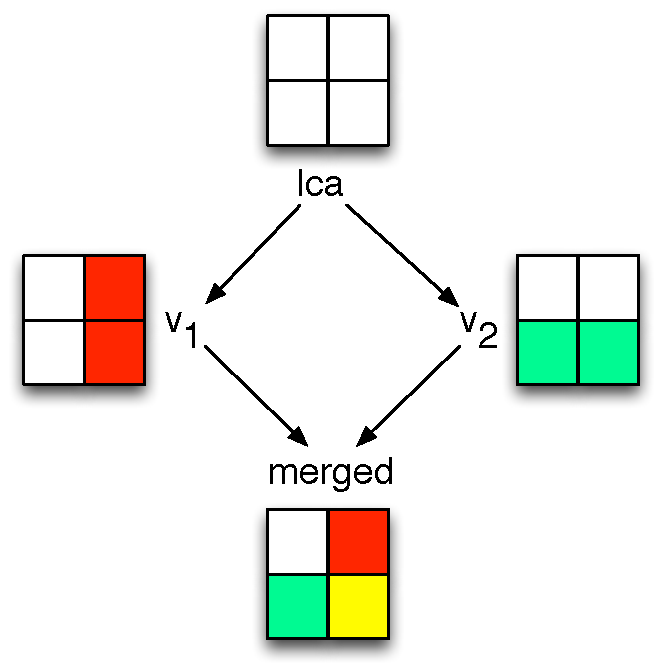
\includegraphics[scale=0.35]{Figures/canvas-merging}
\end{center}
\vspace*{-0.1in}

We have built several mergeable datatypes including lists, ropes, etc, which
can be freely composed together. That is, a list of counters behaves like a
mergeable list for append and remove operations, with updates reconciled
through counter merge semantics.

\section{Distributed Instantiation}

The \name programming model is realized on top of Irmin~\cite{irmin}, an OCaml
library database implementation that is part of the MirageOS
project~\cite{mirage}. Irmin provides a persistent multi-versioned store with a
content-addressable heap abstraction. Simply put, content-addressability means
that the address of a data block is determined by its content. If the content
changes, then so does the address. Old content continues to be available from
the old address. Content-addressability also results in constant time
structural equality checks, which we exploit in our mergeable rope
implementation, among others.

Irmin provides support for distribution, fault-tolerance and concurrency
control by incorporating the Git distributed version control~\cite{git}
protocol over its object model. Indeed, Irmin is fully compatible with Git
command line tools. Distributed replicas in \name are created by cloning a
\name repository. Due to \name's support for mergeable types, each replica can
operate completely independently, accepting client requests, even when
disconnected from other replicas, resulting in a highly available distributed
system.

While Irmin's merge functions are defined over objects on Irmin's
content-addressable heap, \name's merge functions are defined over OCaml types.
We address this representational mismatch with the help of OCaml's PPX
metaprogramming support~\cite{ppx} to derive bi-directional transformations
between objects on OCaml and Irmin heaps. We also derive the various
serialization functions required by Irmin

\begin{figure}[t]
  \centering
	\begin{subfigure}{0.45\columnwidth}
		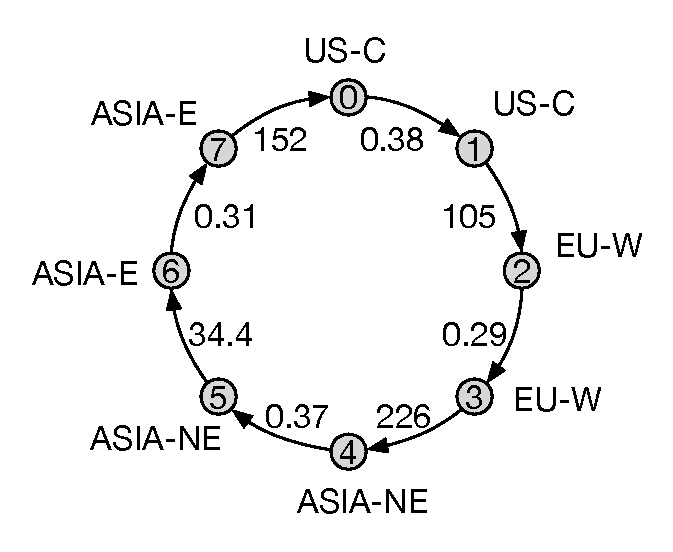
\includegraphics[width=0.9\textwidth]{Figures/cluster.pdf}
		\caption{{\small Our experimental configuration consists of an 8-node ring cluster
			executing on Google Cloud Platform. Edge labels are inter-node latencies in milliseconds.}}
		\label{fig:cluster}
	\end{subfigure}
	\hfill
	\begin{subfigure}{0.5\columnwidth}
		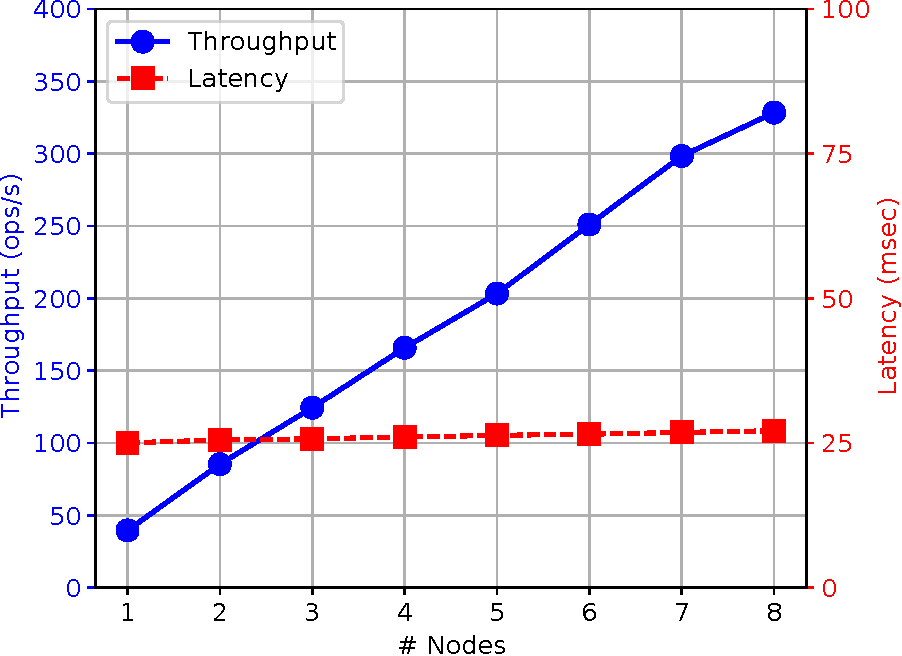
\includegraphics[width=\textwidth]{Figures/scalability.pdf}
		\caption{{\small Scalability: Overall throughput of the cluster and latency of each
		operation.}}
		\label{grf:scalability}
	\end{subfigure}
	\caption{\name performance evaluation.}
  \label{grf:evaluation}
	\vspace{-1em}
\end{figure}

We evaluated the performance of the system on a collaborative application that
simulates concurrent editing of the same document by several authors. The
benchmark itself was constructed with a list of ropes. The workload consists of
4000 edit operations at random indices with 85\% insertions and 15\% deletions.
We evaluate the scalability of concurrent editing application by increasing the
cluster size from 1 to 8 (the 4 node ring cluster consists of nodes numbered 0
to 3), with each node performing concurrent edits to the same document. In each
case, we measure the overall cluster throughput and latency of each operation.
The results are presented in Figure~\ref{grf:scalability}. The results show
that the cluster throughput increases linearly with the number of concurrent
editors, while the latency for each operation remains the same. This is because
each operation is performed locally and does not require synchronization with
other nodes. The nodes remain available to accept requests even if the node
gets disconnected. Since the document type is mergeable, eventually when the
node comes back online, the updates are synchronized with the cluster.

\clearpage

\bibliographystyle{abbrv}
\small
\bibliography{all}

\end{document}
